\chapter{Numerical Results}

In this section, we will show our approximation results for mean-reverting CEV model and Heston plus CEV model, we expand this method with corrective terms up to 3. We utilize a symbolic library of \footnote{Codes used for this paper can be accessed through my \href{https://github.com/ywang408/master-thesis-code}{github}}{python} \href{https://www.sympy.org/en/index.html}{sympy} to apply expansions, and Monte Carlo simulations with 200 steps and 100000 paths as our benchmark because there's no existing pricing formula for these models. To evaluate the accuracy of our results, we use two kinds of figures, the first kind is the direct comparison between benchmarks and our approximation results, the second one is the relative differences between benchmarks and our results. Besides, we also attach detailed results in the Appendix \ref{mrcev}.

\section{Volatility option prices under mean-reverting CEV model}

For options under mean-reverting CEV model,

\begin{equation}\label{numerical1}
  \begin{cases}
    d V_t=\kappa(m - V_t) d t+\sigma_{\text{CEV}} V^{\gamma}_t d W_t &\text{true model}\\
    d V_t=\kappa(m - V_t) d t+\sigma_{\text{CEV}}V_0^{\gamma-\frac{1}{2}} \sqrt{V_t} d W_t &\text{auxiliary model}
  \end{cases}
\end{equation}

\noindent we use the same mean-reverting parameters as \cite{grunbichler_valuing_1996} used in his model, the parameters are $\kappa=4$, $\theta=2$. Besides, we set the nuisance parameter $\sigma_0 = \sigma_{\text{CEV}} V_0^{\gamma-\frac{1}{2}}$, where $V_0=V(t)$, which is the initial value of volatility at time t, see equation \eqref{numerical1}. We test our approximation method with different constant elasticity parameters, the main idea of setting these parameters is that for small $\gamma$, which enlarges the importance of $V$ in the CEV part, we use a small $\sigma$; Whereas for large $\gamma$ we set a large $\sigma$. 

For figure \ref{mrcev res1} and figure \ref{mrcev res2}, our parameters are $\sigma=0.15$, $\gamma=0.3$, and with different maturities $T=0.3$, $T=0.5$. We can find that in \ref{price comparison1} and \ref{price comparison2} our results with corrective terms $N=3$ are very accurate; Figure \ref{price diff1} and figure \ref{price diff2} show the relative error with different corrective terms. We can find that the results with highest corrective terms outperform other results, which implies that keep applying Ito-Taylor expansions on the mis-pricing formula can create increasingly improved refinements and provide us with more and more accurate results.

\begin{figure}[ht]
    \centering
    \subfloat[price comparison]{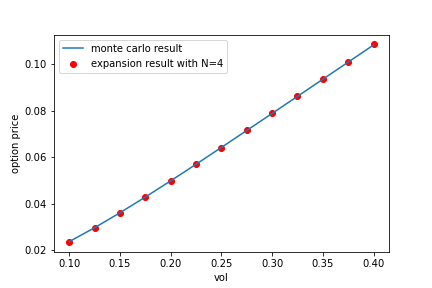
\includegraphics[width=0.5\textwidth]{./figures/T=0.3,K=0.15, kappa=4,m=0.2, sigma=0.15, gamma=0.3.csv price.png}\label{price comparison1}}
    \hfill
    \subfloat[relative error]{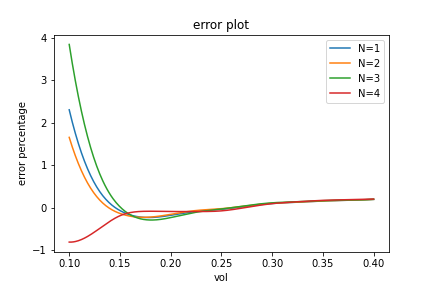
\includegraphics[width=0.5\textwidth]{./figures/T=0.3,K=0.15, kappa=4,m=0.2, sigma=0.15, gamma=0.3.csv error.png}\label{price diff1}}
    \caption{Parameters are $T=0.3,K=0.15, \kappa=4,\theta=0.2, \sigma=0.15, \gamma=0.3$}
  \end{figure}\label{mrcev res1}

\begin{figure}[ht]
  \centering
  \subfloat[price comparison]{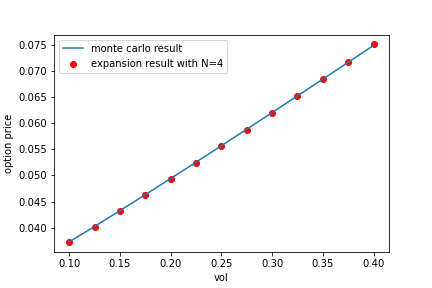
\includegraphics[width=0.5\textwidth]{./figures/T=0.5,K=0.15, kappa=4,m=0.2, sigma=0.15, gamma=0.3.csv price.png}\label{price comparison2}}
  \hfill
  \subfloat[relative error]{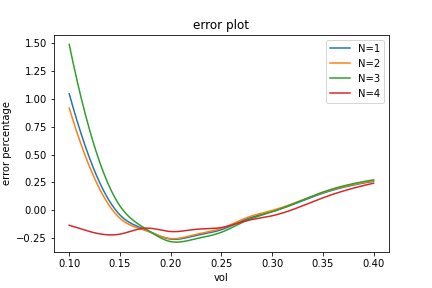
\includegraphics[width=0.5\textwidth]{./figures/T=0.5,K=0.15, kappa=4,m=0.2, sigma=0.15, gamma=0.3.csv error.png}\label{price diff2}}
  \caption{Parameters are $T=0.5,K=0.15, \kappa=4,\theta=0.2, \sigma=0.15, \gamma=0.3$}
\end{figure}\label{mrcev res2}

Parameters for figure \ref{price comparison3} and figure \ref{price comparison4},our parameters are $\sigma=0.6$, $\gamma=0.75$, and with different maturities $T=0.3$, $T=0.5$. Similarly, our method still provide accurate results.

\begin{figure}[ht]
  \centering
  \subfloat[price comparison]{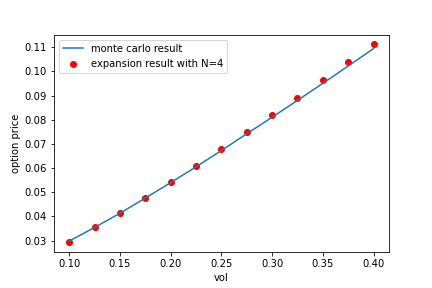
\includegraphics[width=0.5\textwidth]{./figures/T=0.3,K=0.15, kappa=4,m=0.2, sigma=0.6, gamma=0.75.csv price.png}\label{price comparison3}}
  \hfill
  \subfloat[relative error]{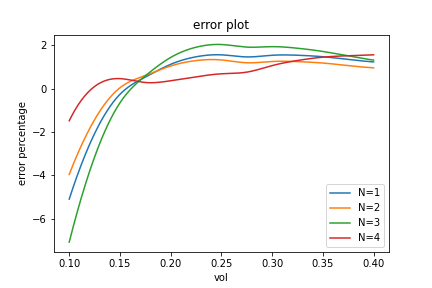
\includegraphics[width=0.5\textwidth]{./figures/T=0.3,K=0.15, kappa=4,m=0.2, sigma=0.6, gamma=0.75.csv error.png}\label{price diff3}}
  \caption{Parameters are $T=0.3,K=0.15, \kappa=4,\theta=0.2, \sigma=0.6, \gamma=0.75$}
\end{figure}

\begin{figure}[ht]
    \centering
    \subfloat[price comparison]{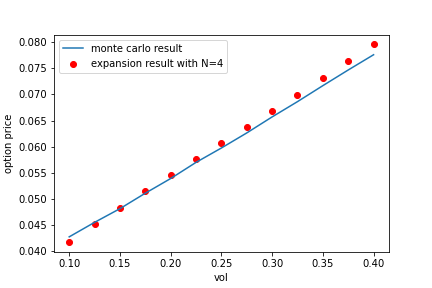
\includegraphics[width=0.5\textwidth]{./figures/T=0.5,K=0.15, kappa=4,m=0.2, sigma=0.6, gamma=0.75.csv price.png}\label{price comparison4}}
    \hfill
    \subfloat[relative error]{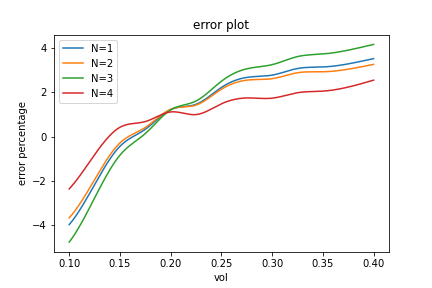
\includegraphics[width=0.5\textwidth]{./figures/T=0.5,K=0.15, kappa=4,m=0.2, sigma=0.6, gamma=0.75.csv error.png}\label{price diff4}}
    \caption{Parameters are $T=0.5,K=0.15, \kappa=4,\theta=0.2, \sigma=0.6, \gamma=0.75$}
\end{figure}


One may observe that when KM use Black-Scholes model as auxiliary model to price options under Heston model, for deep in-the-money options, relative error always converge to 0 no matter how many corrective terms are applied. That is because in his case delta of option is very close to 1 and vega is close to 0, which means option prices are mainly driven by underlying stocks' prices, and volatility has no influence on option prices. Besides, using Black-Scholes model makes mis-pricing term depend on gamma, while gamma of deep in-the-money options is also close to 0, meaning that their mis-pricing terms don't affect option prices at all. As a result, their figures show that all results' relative errors are converging to 0 as stock price increases.

However, in our model, underlying assets follow mean-reverting CEV model. \cite{grunbichler_valuing_1996} mention that when volatility $V$ is above its long-term mean, mean-reversion property implies the expected future value of V will be lower than its current value, making the expected payoff for a volatility call can be less than its current intrinsic value. The property of options under Black-Scholes world doesn't hold here, recall that before we set $\sigma_0 = \sigma_{\text{CEV}}v_0^{\gamma-\frac{1}{2}}$. Obviously when $V_0$ is large, $\sigma_{\text{CEV}} V^{\gamma}_t < \sigma_{\text{CEV}}V_0^{\gamma-\frac{1}{2}} \sqrt{V}_t$, causing the loss of accuracy in our auxiliary model. It gives an explanation why the relative error of our method is slightly larger than 0 for deep in-the-money options. Additionally, using our method to price deep out-of-money options can also be challenging. The loss of accuracy for approximating non-central chi-square distribution functions would be magnified when option price is very small.


\section{Volatility option prices under Heston puls CEV model}

For Heston plus CEV model, our parameters are $r=0.05$, $K=0.15$,$\kappa_1=4$, $\kappa_2=2$, $\theta_2=0.2$, $\sigma_1=0.3$, $\sigma_2=0.8$, $\gamma=1.6$, $\rho=0.5$ and different maturities $T-t=0.3, T-t=0.5$. We set the nuisance parameters $\theta_0 = \theta$, where $V_2(t)=0.2$ is the spot value for volatility of volatility at time $t$.

\begin{figure}[ht]
  \centering
  \subfloat[price comparison]{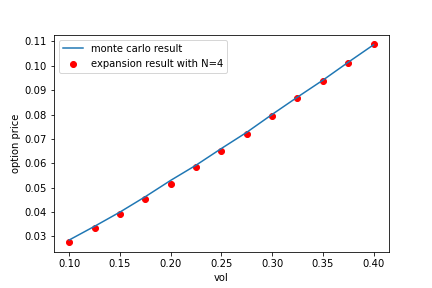
\includegraphics[width=0.5\textwidth]{./figures/heston cev T=0.3,K=0.15, kappa=4,kappa2 =2,theta=0.2, sigma1=0.3,sigam2=0.8, gamma=1.6.csv price.png}\label{2d price comparison1}}
  \hfill
  \subfloat[relative error]{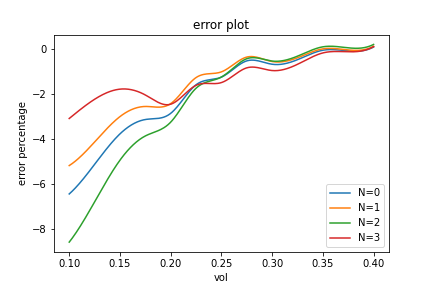
\includegraphics[width=0.5\textwidth]{./figures/heston cev T=0.3,K=0.15, kappa=4,kappa2 =2,theta=0.2, sigma1=0.3,sigam2=0.8, gamma=1.6.csv error.png}\label{2d price diff1}}
  \caption{Heston plus CEV model result 1}
\end{figure}

\begin{figure}[ht]
  \centering
  \subfloat[price comparison]{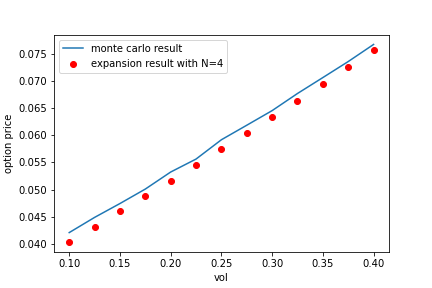
\includegraphics[width=0.5\textwidth]{./figures/heston cev T=0.5,K=0.15, kappa=4,kappa2 =2,theta=0.2, sigma1=0.3,sigam2=0.8, gamma=1.6.csv price.png}\label{2d price comparison2}}
  \hfill
  \subfloat[relative error]{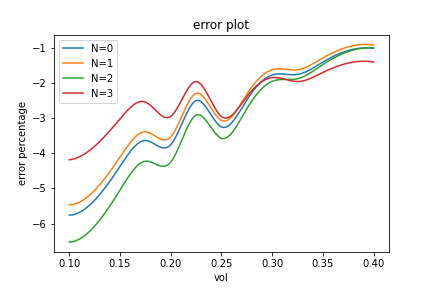
\includegraphics[width=0.5\textwidth]{./figures/heston cev T=0.5,K=0.15, kappa=4,kappa2 =2,theta=0.2, sigma1=0.3,sigam2=0.8, gamma=1.6.csv error.png}\label{2d price diff2}}
  \caption{Heston plus CEV model result 2}
\end{figure}

As is seen in \ref{2d price comparison1}, applying our method under 2-dimensional model can still create relatively accurate results. Unlike mean-reverting CEV model, under Heston plus CEV model our relative error is now converging to 0. This is because here the initial value of volatility doesn't enter mis-pricing term $\delta = \kappa_1(V_2-\theta_2) \Delta_{\bar{w}}$.

Besides, we notice that for \ref{2d price comparison2} when $T=0.5$, our results aren't accurate compared to other situations. Though in this case results become more accurate as we take more corrective terms. We may predict that if applying higher order expansions we could get more precise results. However, this raises a limit of KM's method, number of terms grow exponentially in the final pricing formula as we apply higher order expansions, causing the running time of calculation increasing dramatically. Such condition leads to reconsidering nuisance parameters and auxiliary models.

\chapter{Conclusion}

In this paper, we introduce approximation method proposed by \cite{david_variance_nodate} and \cite{kristensen_adding_2011}. Based on their work, we extend this method to price options under mean-reverting CEV model and Heston plus CEV models. Selections of auxiliary models and corresponding mis-pricing formula are discussed, we also illustrate techniques to calculate partial derivatives of non-central chi-square distribution functions when using square root mean-reverting as auxiliary model. Finally, we discuss our numerical results and explain the constraints of our method. In all, numerical results show that our method is efficient and accurate.